\chapter{Mutable objects}
\label{chap08}
\label{objects}
\index{object}


%\section{{\tt Point}s and {\tt Rectangle}s}
\index{String}
\index{type!String}

{\tt String}s are objects, but they are atypical objects
because

\begin{itemize}

\item They are immutable.

\item They have no attributes.

\item You don't have to use {\tt new} to create one.

\end{itemize}

In this chapter, we use two objects from Java libraries,
 {\tt Point} and {\tt Rectangle}.
But first, I want to make it clear that these points
and rectangles are not graphical objects that appear on the
screen.  They are values that contain data, just like {\tt int}s
and {\tt double}s.  Like other values, they are used internally
to perform computations.


%\index{AWT}
%\index{Abstract Window Toolkit|see {AWT}}

%, and {\tt java.awt}, the {\bf Abstract Window Toolkit} (AWT), which contains classes for windows, buttons, graphics, etc.

% {\tt Point} and {\tt Rectangle} are in the {\tt java.awt} package, so to import them like this:


\section{{\tt Point} objects}
\index{Point}
\index{class!Point}

A point is two numbers (coordinates)
that we treat collectively as a single object.  In mathematical
notation, points are often written in parentheses, with a comma
separating the coordinates.  For example, $(0, 0)$ indicates
the origin, and $(x, y)$ indicates the point $x$ units to the
right and $y$ units up from the origin.

\index{new}
\index{statement!new}

In Java, a point is represented by a {\tt Point} object.  To
create a new point, you have to use {\tt new}:

\begin{code}
    Point blank;
    blank = new Point(3, 4);
\end{code}
%
The first line is a conventional variable declaration: {\tt blank}
has type {\tt Point}.  The second line invokes {\tt new}, specifies
the type of the new object, and provides arguments.  The arguments are
the coordinates of the new point, $(3, 4)$.

\index{declaration}
\index{statement!declaration}
\index{reference}
\index{state diagram}
\index{state}

The result of {\tt new} is a {\bf reference} to the new
point, so {\tt blank} contains a reference to the
newly-created object.  There is a standard way to diagram this
assignment, shown in the figure.


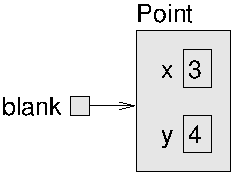
\includegraphics{figs/reference.pdf}


As usual, the name of the variable {\tt blank} appears outside the box
and its value appears inside the box.  In this case, that value is a
reference, which is shown graphically with an arrow.  The
arrow points to the object we're referring to.

The big box shows the newly-created object with the two values
in it.  The names {\tt x} and {\tt y} are the names of the {\bf
instance variables}.

Taken together, all the variables, values, and objects in a
program are called the {\bf state}.  Diagrams like this that
show the state of the program are called {\bf state diagrams}.
As the program runs, the state changes, so you should think
of a state diagram as a snapshot of a particular point in the
execution.


\section{Instance variables}
\index{variable!instance}
\index{instance variable}

The pieces of data that make up an object are called instance
variables because each object, which is an {\bf instance} of its
type, has its own copy of the instance variables.

It's like the glove compartment of a car.  Each car is an instance
of the type ``car,'' and each car has its own glove compartment.  If
you ask me to get something from the glove compartment of your car,
you have to tell me which car is yours.

\index{dot notation}

Similarly, if you want to read a value from an instance variable, you
have to specify the object you want to get it from.  In Java this is
done using ``dot notation.''

\begin{code}
    int x = blank.x;
\end{code}
%
The expression {\tt blank.x} means ``go to the object {\tt blank}
refers to, and get the value of {\tt x}.''  In this case we assign
that value to a local variable named {\tt x}.  There is no
conflict between the local variable named {\tt x} and the instance
variable named {\tt x}.  The purpose of dot notation is to identify
{\em which} variable you are referring to unambiguously.

You can use dot notation as part of any Java expression, so the
following are legal.

\begin{code}
    System.out.println(blank.x + ", " + blank.y);
    int distance = blank.x * blank.x + blank.y * blank.y;
\end{code}
%
The first line prints {\tt 3, 4}; the second line calculates
the value 25.

\section{Objects as parameters}
\index{parameter}
\index{object!as parameter}

You can pass objects as parameters in the usual way.  For
example:

\begin{code}
  public static void printPoint(Point p) {
    System.out.println("(" + p.x + ", " + p.y + ")");
  }
\end{code}
%
This method takes a point as an argument and prints it in
the standard format.  If you invoke {\tt printPoint(blank)},
it prints {\tt(3, 4)}.  Actually, Java already has a
method for printing {\tt Points}.  If you invoke
{\tt System.out.println(blank)}, you get

\begin{code}
java.awt.Point[x=3,y=4]
\end{code}
%
This is a standard format Java uses for printing objects.  It prints
the name of the type, followed by the names and values of the instance
variables.

As a second example, we can rewrite the {\tt distance} method from
Section~\ref{distance} so that it takes two {\tt Point}s as parameters
instead of four {\tt double}s.

\begin{code}
  public static double distance(Point p1, Point p2) {
    double dx = (double)(p2.x - p1.x);
    double dy = (double)(p2.y - p1.y);
    return Math.sqrt(dx*dx + dy*dy);
  }
\end{code}
%
The typecasts are not really necessary; I added them as a
reminder that the instance variables in a {\tt Point} are integers.


\section{Rectangles}
\index{Rectangle}
\index{class!Rectangle}

{\tt Rectangle}s are similar to points, except that they have four
instance variables: {\tt x}, {\tt y}, {\tt width} and {\tt
height}.  Other than that, everything is pretty much the same.

This example
creates a {\tt Rectangle} object and makes {\tt box} refer to it.

\begin{code}
    Rectangle box = new Rectangle(0, 0, 100, 200);
\end{code}
%
This figure shows the effect of this assignment.


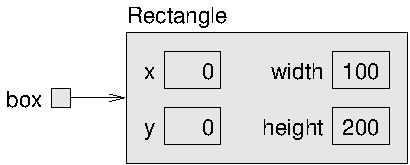
\includegraphics{figs/rectangle.pdf}

If you print {\tt box}, you get

\begin{code}
java.awt.Rectangle[x=0,y=0,width=100,height=200]
\end{code}
%
Again, this is the result of a Java method that knows how
to print {\tt Rectangle} objects.


\section{Objects as return types}
\index{object!as return type}
\index{return}
\index{statement!return}

You can write methods that return objects.  For example,
{\tt findCenter} takes a {\tt Rectangle} as an argument and
returns a {\tt Point} that contains the coordinates of the
center of the {\tt Rectangle}:

\begin{code}
  public static Point findCenter(Rectangle box) {
    int x = box.x + box.width/2;
    int y = box.y + box.height/2;
    return new Point(x, y);
  }
\end{code}
%
Notice that you can use {\tt new} to create a new object,
and then immediately use the result as the return value.


\section{Objects are mutable}
\index{object!mutable}
\index{mutable}

You can change the contents of an object by making an assignment
to one of its instance variables.  For example, to ``move''
a rectangle without changing its size, you can modify the
{\tt x} and {\tt y} values:

\begin{code}
    box.x = box.x + 50;
    box.y = box.y + 100;
\end{code}
%
The result is shown in the figure:


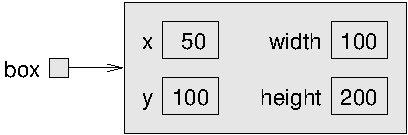
\includegraphics{figs/rectangle2.pdf}


\index{encapsulation}
\index{generalization}

We can encapsulate this code in a method and
generalize it to move the rectangle by any amount:

\begin{code}
  public static void moveRect(Rectangle box, int dx, int dy) {
    box.x = box.x + dx;
    box.y = box.y + dy;
  }
\end{code}
%
The variables {\tt dx} and {\tt dy} indicate how far to move the
rectangle in each direction.  Invoking this method has the effect of
modifying the {\tt Rectangle} that is passed as an argument.

\begin{code}
    Rectangle box = new Rectangle(0, 0, 100, 200);
    moveRect(box, 50, 100);
    System.out.println(box);
\end{code}
%
prints {\tt java.awt.Rectangle[x=50,y=100,width=100,height=200]}.

Modifying objects by passing them as arguments to methods can be
useful, but it can also make debugging more difficult because it is
not always clear which method invocations do or do not modify their
arguments.  Later, I discuss some pros and cons of this
programming style.

Java provides methods that operate on Points and Rectangles.  You can
read the documentation at
\url{http://download.oracle.com/javase/6/docs/api/java/awt/Point.html}
and
\url{http://download.oracle.com/javase/6/docs/api/java/awt/Rectangle.html}.

For example, {\tt translate} has the same effect as {\tt moveRect},
but instead of passing the Rectangle as an argument, you use dot
notation:

\begin{code}
    box.translate(50, 100);
\end{code}
%
%The effect is the same.


\section{Aliasing}
\label{aliasing}
\index{aliasing}
\index{reference}

Remember that when you assign an object to a variable, you
are assigning a {\em reference} to an object.  It is possible to have
multiple variables that refer to the same object.  For example,
this code:

\begin{code}
    Rectangle box1 = new Rectangle(0, 0, 100, 200);
    Rectangle box2 = box1;
\end{code}
%
generates a state diagram that looks like this:


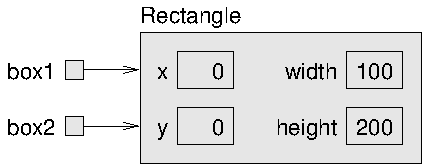
\includegraphics{figs/aliasing.pdf}


{\tt box1} and {\tt box2} refer to the same object.
In other words, this object has two names, {\tt box1} and {\tt box2}.
When a person uses two names, it's called {\bf aliasing}.  Same thing
with objects.

When two variables are aliased, any changes that affect one
variable also affect the other.  For example:

\begin{code}
    System.out.println(box2.width);
    box1.grow(50, 50);
    System.out.println(box2.width);
\end{code}
%
The first line prints {\tt 100}, which is the width of the
{\tt Rectangle} referred to by {\tt box2}.  The second
line invokes the {\tt grow} method on {\tt box1}, which
expands the {\tt Rectangle} by 50 pixels in every direction
(see the documentation for more details).  The effect
is shown in the figure:


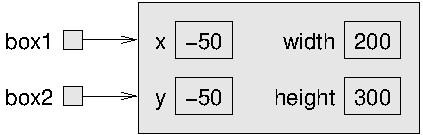
\includegraphics{figs/aliasing2.pdf}


Whatever changes are
made to {\tt box1} also apply to {\tt box2}.  Thus, the
value printed by the third line is {\tt 200}, the width of
the expanded rectangle. (As an aside, it is perfectly legal
for the coordinates of a {\tt Rectangle} to be negative.)

As you can tell even from this simple example, code that
involves aliasing can get confusing fast, and can be
difficult to debug.  In general, aliasing should be avoided
or used with care.


\section{{\tt null}}
\index{null}

When you create an object variable, remember that you are
creating a {\em reference} to an object.  Until you make
the variable point to an object, the value of the variable
is {\tt null}.  {\tt null} is a special value (and
a Java keyword) that means ``no object.''

The declaration {\tt Point blank;} is equivalent to this
initialization

\begin{code}
    Point blank = null;
\end{code}
%
and is shown in the following state diagram:



\includegraphics{figs/reference2.pdf}


The value {\tt null} is represented by a small square with no arrow.

\index{exception!NullPointer}
\index{run-time error}

If you try to use a null object, either by accessing an instance
variable or invoking a method, Java throws a {\tt
NullPointerException}, prints an error message
and terminates the program.

\begin{code}
    Point blank = null;
    int x = blank.x;              // NullPointerException
    blank.translate(50, 50);      // NullPointerException
\end{code}
%
On the other hand, it is legal to pass a null object as an argument or
receive one as a return value.  In fact, it is common to do so, for
example to represent an empty set or indicate an error condition.


\section{Garbage collection}
\index{garbage collection}

In Section~\ref{aliasing} we talked about what happens when
more than one variable refers to the same object.  What happens
when {\em no} variable refers to an object?  For example:

\begin{code}
    Point blank = new Point(3, 4);
    blank = null;
\end{code}
%
The first line creates a new {\tt Point} object and makes
{\tt blank} refer to it.  The second line changes {\tt blank}
so that instead of referring to the object, it refers to
nothing (the null object).


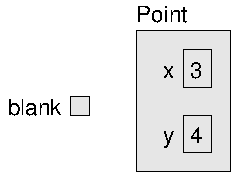
\includegraphics{figs/reference3.pdf}


If no one refers to an object, then no one can read or write any of
its values, or invoke a method on it.  In effect, it ceases to exist.
We could keep the object in memory, but it would only waste space, so
periodically as your program runs, the system looks for stranded
objects and reclaims them, in a process called {\bf garbage
collection}.  Later, the memory space occupied by the object will
be available to be used as part of a new object.

You don't have to do anything to make garbage collection happen,
and in general you will not be aware of it.  But you
should know that it periodically runs in the background.


\section{Objects and primitives}
\index{type!object}
\index{type!primitive}
\index{object type}
\index{primitive type}

There are two kinds of types in Java, primitive types and
object types.  Primitives, like {\tt int} and {\tt boolean}
begin with lower-case letters; object types begin with
upper-case letters.  This distinction is useful because it
reminds us of some of the differences between them:

\begin{itemize}

\item When you declare a primitive variable, you get storage
space for a primitive value.  When you declare an object variable, you
get a space for a reference to an object.  To get space for
the object itself, you have to use {\tt new}.

\item If you don't initialize a primitive type, it is given
a default value that depends on the type.  For example,
{\tt 0} for {\tt int}s and {\tt false} for {\tt boolean}s.
The default value for object types is {\tt null}, which indicates
no object.

\item Primitive variables are well isolated in the sense that there is
nothing you can do in one method that will affect a variable in
another method.  Object variables can be tricky to work with because
they are not as well isolated.  If you pass a reference to an object
as an argument, the method you invoke might modify the object, in which
case you will see the effect.  Of course, that can be a good thing, but you
have to be aware of it.

\end{itemize}

There is one other difference between primitives and object
types.  You cannot add new primitives to Java
(unless you get yourself on the standards committee), but
you can create new object types!  We'll see how in the next
chapter.

\section{Glossary}

\begin{description}

\item[AWT:]  The Abstract Window Toolkit, one of the biggest
and commonly-used Java packages.

\item[instance:]  An example from a category.  My cat is an
instance of the category ``feline things.''  Every object is
an instance of some class.

\item[instance variable:]  One of the named data items that make
up an object.  Each object (instance) has its own copy of
the instance variables for its class.

\item[reference:]  A value that indicates an object.  In a
state diagram, a reference appears as an arrow.

\item[aliasing:] The condition when two or more variables refer
to the same object.

\item[garbage collection:]  The process of finding objects that
have no references and reclaiming their storage space.

\item[state:] A complete description of all the variables and
objects and their values, at a given point during the execution
of a program.

\item[state diagram:] A snapshot of the state of a program, shown
graphically.

\index{instance}
\index{instance variable}
\index{reference}
\index{aliasing}
\index{garbage collection}
\index{state}
\index{state diagram}

\end{description}


\section{Exercises}

\begin{exercise}
\begin{enumerate}

\item For the following program, draw a stack diagram showing the
local variables and parameters of {\tt main} and {\tt riddle}, and show
any objects those variables refer to.

\item What is the output of this program?

\end{enumerate}

\begin{code}
public static void main(String[] args)
{
    int x = 5;
    Point blank = new Point(1, 2);

    System.out.println(riddle(x, blank));
    System.out.println(x);
    System.out.println(blank.x);
    System.out.println(blank.y);
}

public static int riddle(int x, Point p)
{
    x = x + 7;
    return x + p.x + p.y;
}
\end{code}

The point of this exercise is to make sure you understand the
mechanism for passing Objects as parameters.
\end{exercise}


\begin{exercise}
\begin{enumerate}

\item For the following program, draw a stack diagram showing the
state of the program just before {\tt distance} returns.  Include all
variables and parameters and the objects those variables refer to.

\item What is the output of this program?

\end{enumerate}

\begin{code}
public static double distance(Point p1, Point p2) {
    int dx = p1.x - p2.x;
    int dy = p1.y - p2.y;
    return Math.sqrt(dx*dx + dy*dy);
}

public static Point findCenter(Rectangle box) {
    int x = box.x + box.width/2;
    int y = box.y + box.height/2;
    return new Point(x, y);
}

public static void main(String[] args) {
    Point blank = new Point(5, 8);

    Rectangle rect = new Rectangle(0, 2, 4, 4);
    Point center = findCenter(rect);

    double dist = distance(center, blank);

    System.out.println(dist);
}
\end{code}
%
\end{exercise}



\begin{exercise}
The method {\tt grow} is part of the {\tt Rectangle} class.  Read the
documentation at
\url{http://download.oracle.com/javase/6/docs/api/java/awt/Rectangle.html#grow(int, int)}.

\begin{enumerate}

\item What is the output of the following program?

\item Draw a state diagram that shows the state of the
program just before the end of {\tt main}.
Include all local variables and the objects
they refer to.

\item At the end of {\tt main}, are {\tt p1} and
{\tt p2} aliased?  Why or why not?

\end{enumerate}

\begin{code}
public static void printPoint(Point p) {
    System.out.println("(" + p.x + ", " + p.y + ")");
}

public static Point findCenter(Rectangle box) {
    int x = box.x + box.width/2;
    int y = box.y + box.height/2;
    return new Point(x, y);
}

public static void main(String[] args) {

    Rectangle box1 = new Rectangle(2, 4, 7, 9);
    Point p1 = findCenter(box1);
    printPoint(p1);

    box1.grow(1, 1);
    Point p2 = findCenter(box1);
    printPoint(p2);
}
\end{code}

\end{exercise}


\begin{exercise}
\label{ex.biginteger}
You might be sick of the factorial
method by now, but we're going to do one more version.

\begin{enumerate}

\item Create a new program called {\tt Big.java} and
write an iterative version of {\tt factorial}.

\item Print a table of the integers from 0 to 30 along with their
factorials.  At some point around 15, you will probably see
that the answers are not right any more.  Why not?

\item BigIntegers are Java objects that can represent arbitrarily big
  integers.  There is no upper bound except the limitations of memory
  size and processing speed.  Read the documentation of BigIntegers at
  \url{http://download.oracle.com/javase/6/docs/api/java/math/BigInteger.html}.

\item To use BigIntegers, you have to add {\tt import
java.math.BigInteger} to the beginning of your program.

\item There are several ways to create a
BigInteger, but the one I recommend uses {\tt valueOf}.
The following code converts an integer to a {\tt BigInteger}:

\begin{code}
    int x = 17;
    BigInteger big = BigInteger.valueOf(x);
\end{code}

Type in this code and try it out.  Try printing a BigInteger.

\item Because BigIntegers are not primitive types,
the usual math operators don't work.  Instead we
have to use methods like {\tt add}.  To
add two BigIntegers, invoke {\tt add} on one
and pass the other as an argument.  For example:

\begin{code}
    BigInteger small = BigInteger.valueOf(17);
    BigInteger big = BigInteger.valueOf(1700000000);
    BigInteger total = small.add(big);
\end{code}

Try out some of the other methods, like {\tt multiply} and
{\tt pow}.

\item Convert {\tt factorial} so that it performs its calculation
using BigIntegers and returns a BigInteger as a result.
You can leave the parameter alone---it will still be an integer.

\item Try printing the table again with your modified factorial
method.  Is it correct up to 30?  How high can you make it go?  I
calculated the factorial of all the numbers from 0 to 999, but my
machine is pretty slow, so it took a while.  The last number, 999!,
has 2565 digits.

\end{enumerate}
\end{exercise}

\begin{exercise}
Many encryption techniques depend on the
ability to raise large integers to an integer power.  Here is a
method that implements a (reasonably) fast technique for integer
exponentiation:

\begin{code}
public static int pow(int x, int n) {
    if (n == 0) return 1;

    // find x to the n/2 recursively
    int t = pow(x, n/2);

    // if n is even, the result is t squared
    // if n is odd, the result is t squared times x

    if (n%2 == 0) {
      return t*t;
    } else {
      return t*t*x;
    }
}
\end{code}

The problem with this method is that it only works if the result
is smaller than 2 billion.  Rewrite it so that the result is
a {\tt BigInteger}.  The parameters should still be integers, though.

You can use the BigInteger methods {\tt add} and {\tt multiply}, but
don't use {\tt pow}, which would spoil the fun.
\end{exercise}


\begin{exercise}
If you are interested in graphics, now is a good time to read
Appendix~\ref{graphics} and do the exercises there.
\end{exercise}


